\documentclass[a4paper,12pt]{article}

% Packages
\usepackage[T1]{fontenc}     % Font encoding
\usepackage{lmodern}         % Modern font
\usepackage{geometry}        % Page layout
\geometry{margin=1in}        % 1-inch margins
\usepackage{amsmath,amssymb}  % Math symbols
\usepackage{booktabs}        % Better tables
\usepackage{graphicx}        % Include graphics
\usepackage{setspace}        % Adjust line spacing
\usepackage{titling}         % Customize title format
\usepackage{float}          % For figure placement

% Reduce overall line spacing (adjust the factor as needed)
\setstretch{0.9}

% Title Page adjustments: reduce title size and vertical spacing
\pretitle{\begin{center}\bfseries\Large}    % Change \Large to a smaller size if needed (e.g., \large)
\posttitle{\end{center}\vspace{-1em}}         % Reduce vertical space after title
\preauthor{\begin{center}\small}
\postauthor{\end{center}\vspace{-1em}}
\predate{}
\postdate{}

\title{Report HW1}
\author{%
    \begin{tabular}{cc}
        Simone De Carli & Damiano Salvaterra \\
        {\small \texttt{simone.decarli@studenti.unitn.it}} & {\small \texttt{damiano.salvaterra@studenti.unitn.it}}
    \end{tabular}
}
\date{}  % Empty date

\begin{document}

\maketitle

\newcommand{\E}[1]{\operatorname{E}\left[#1\right]}
\newcommand{\Var}[1]{\operatorname{Var}\left[#1\right]}

\section*{Introduction}

We conducted the following exercises with \(10^7\) samples for each experiment.

We also used 5 different RNGs: (\texttt{MT19937}, \texttt{PCG64}, \texttt{PCG64DXSM}, \texttt{Philox}, \texttt{SFC64}) provided by the \texttt{numpy} library.

\section*{Exercise 1}

% Gaussians parameters:

% \begin{center}
% \begin{tabular}{c|cc|c}
%     \toprule
%     \textbf{N°} & \textbf{Mean} & \textbf{Variance} & \textbf{Probability} \\
%     \midrule
%     1 & -2 & 2 & 0.15 \\
%     2 & 4  & 1 & 0.25 \\
%     3 & 10 & 3 & 0.35 \\
%     4 & 15 & 2 & 0.25 \\
%     \bottomrule
% \end{tabular}
% \end{center}

Let \(X\) be the random variable representing the drawn number from one of the four Gaussians, and let \(Y\) be the random variable representing the Gaussian from which the number is drawn.

The expectation of \(X\) can be calculated as follows:
\begin{equation*}\begin{split}
		\E{X} &= \E{X \mid Y=1}P(Y=1) + \E{X \mid Y=2}P(Y=2)\\
		&\quad + \E{X \mid Y=3}P(Y=3) + \E{X \mid Y=4}P(Y=4) \\
		&= 7.95.
	\end{split}
\end{equation*}

The variance of \(X\) can be calculated as follows:
\begin{equation*}
	\begin{split}
		\Var{X} &= \E{\Var{X \mid Y}} + \Var{\E{X \mid Y}} \\
		&= \sigma^2_1 \cdot P(Y=1) + \sigma^2_2 \cdot P(Y=2) + \sigma^2_3 \cdot P(Y=3) + \sigma^2_4 \cdot P(Y=4) \\
		&\quad + \E{\E{X \mid Y}^2} - \E{X}^2 \\
		&= 34.7475.
	\end{split}
\end{equation*}

\begin{figure}[H]
	\centering
	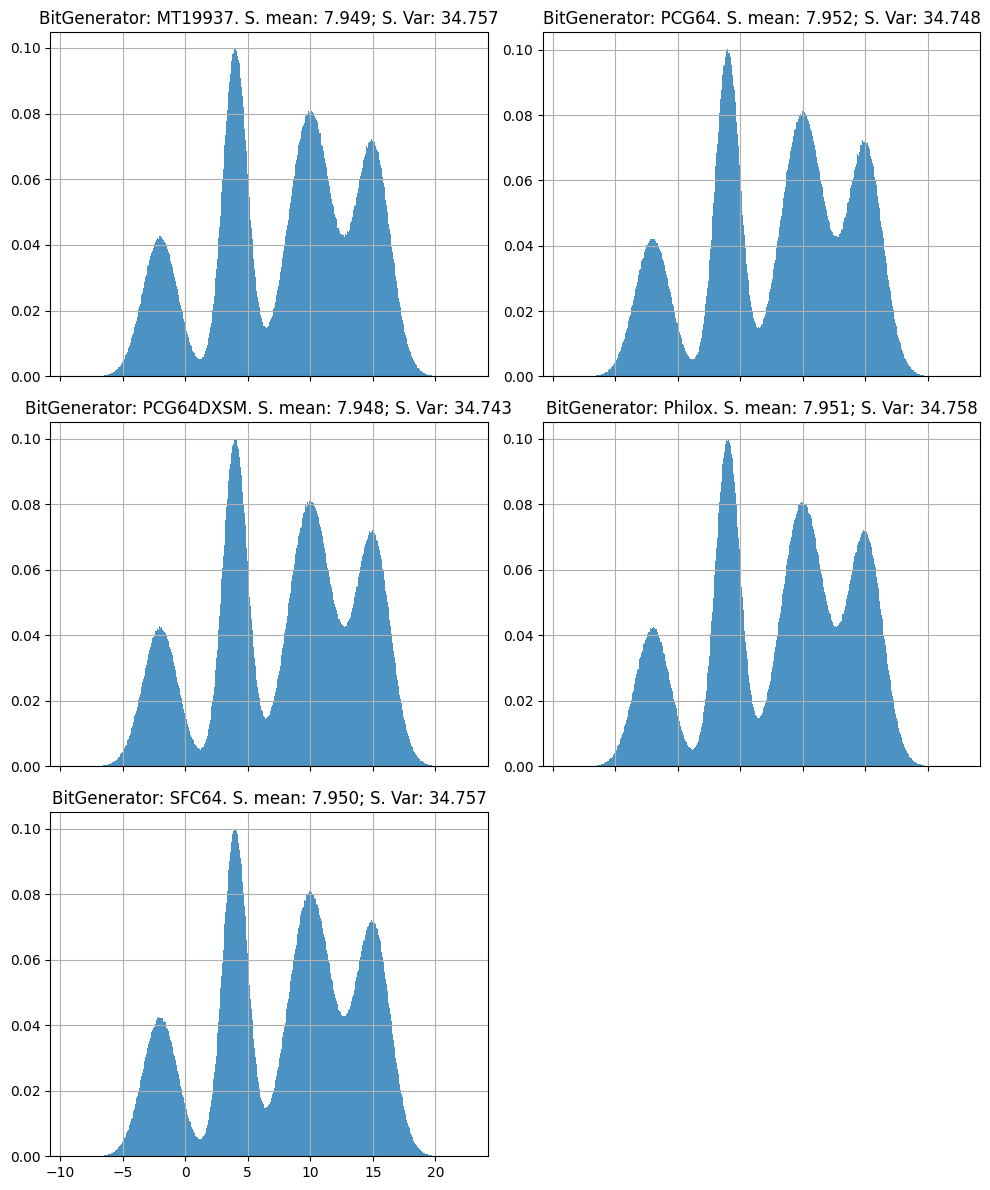
\includegraphics[width=1\textwidth]{ex1-plot.png}
	\caption{Density plot of the samples drawn from the four Gaussians.}
\end{figure}

\section*{Exercise 2}

Let \(X \sim \operatorname{Exp}(\lambda)\) and \(Y \sim U(a,b)\). We wish to calculate the probability:
\[
	P(X > Y).
\]

Since \(X\) and \(Y\) are independent, we can write:
\[
	P(X > Y) = \int_a^b P(X > y \mid Y = y) f_Y(y) \, dy,
\]
where \(f_Y(y)\) is the density of the uniform distribution on \([a,b]\):
\[
	f_Y(y) = \frac{1}{b-a}, \quad \text{for } y \in [a,b].
\]

For an exponential random variable \(X\) with parameter \(\lambda\), the survival function is:
\[
	P(X > y) = \int_y^\infty \lambda e^{-\lambda x} \, dx = e^{-\lambda y}, \quad \text{for } y \ge 0.
\]

Substituting the expression for \(P(X > y)\) into the integral:
\[
	P(X > Y) = \frac{1}{b-a} \int_a^b e^{-\lambda y} \, dy.
\]
We compute the integral:
\[
	\int_a^b e^{-\lambda y} \, dy = \left[ -\frac{1}{\lambda} e^{-\lambda y} \right]_a^b = \frac{1}{\lambda}\left(e^{-\lambda a} - e^{-\lambda b}\right).
\]
We finally obtain:
\[
	P(X > Y) = \frac{e^{-\lambda a} - e^{-\lambda b}}{\lambda (b-a)}.
\]
Thus, the final expression is:
\[
	\boxed{P(X > Y) = \frac{e^{-\lambda a} - e^{-\lambda b}}{\lambda (b-a)}.}
\]

Setting \(\lambda=1\), \(a=0\), and \(b=5\), we have:
\[
	P(X > Y) = \frac{1 - e^{-5}}{5} \approx 0.1987.
\]

\begin{figure}[h]
	\centering
	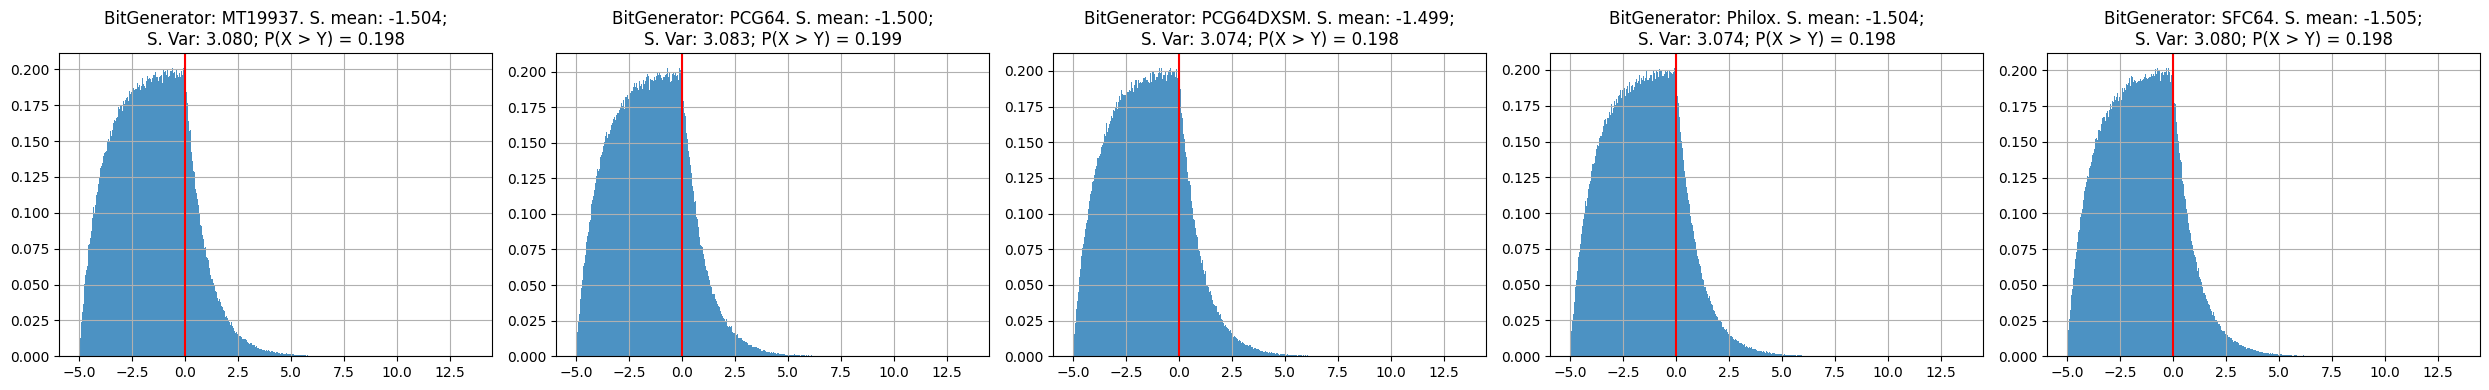
\includegraphics[width=1\textwidth]{ex2-plot.png}
	\caption{Density plot of the difference between the exponential and uniform distributions.}
\end{figure}

\end{document}
